\documentclass[a4paper, twoside]{report}
%% Language and font encodings
\usepackage[english]{babel}
\usepackage[utf8x]{inputenc}
\usepackage[T1]{fontenc}

%% Chapter Beautify
\usepackage{titlesec}
% \newcommand{\hsp}{\hspace{20pt}}
% \titleformat{\chapter}[hang]{\Huge\bfseries}{\thechapter\hsp|\hsp}{0pt}{\Huge\bfseries}

%% Very nice Font
\usepackage{palatino}

%% Diagram drawing
\usepackage{tikz}
\usetikzlibrary{shapes.geometric, arrows}

%% Forced float
\usepackage{float}

%% Source code highlight
\usepackage{minted}
\usepackage{listings}

%% Code line references
\setminted[haskell]{escapeinside=\#\#, linenos=true, mathescape=true}
\usepackage{caption}
\usepackage{tikz}
\newcommand*\circled[1]{\tikz[baseline=(char.base)]{
            \node[shape=circle,draw,inner sep=1pt, text=white] (char) {#1};}}
\newcommand*\clabel[1]{$\label{#1} \circled{\ref{#1}}$}
\newcommand*\cref[1]{\circled{\ref{#1}}}
\newcommand*\ccaption[2]{
    \caption[.]{
        \centering #1\newline
        \begin{minipage}{\linewidth}
            #2
        \end{minipage}
        \newline
    }
}

\newenvironment{code}{\captionsetup{type=listing}}{}
%% Automatic Reference

% BNF Rule
\usepackage{mathtools,array}
\newenvironment{grammar}[2]
 {\begin{tabular}{@{\qquad}>{$}l<{$}@{\qquad}l@{}}
  \multicolumn{1}{@{}l@{}}{$#1$}&\multicolumn{1}{l@{}}{\hspace{-2em}#2}\\}
 {\end{tabular}}

%% Placeholder picture
\usepackage{mwe}

%% Format Paragraph
\setcounter{secnumdepth}{4}
\titleformat{\paragraph}
{\normalfont\normalsize\bfseries}{\theparagraph}{1em}{}
\titlespacing*{\paragraph}
{0pt}{3.25ex plus 1ex minus .2ex}{1.5ex plus .2ex}

%% Sets page size and margins
\usepackage[a4paper,top=3cm,bottom=2cm,left=3cm,right=3cm,marginparwidth=1.75cm]{geometry}

%% Useful packages
\usepackage{amsmath}
\usepackage{amssymb}
\usepackage{graphicx}
\usepackage{subcaption}
\usepackage[colorinlistoftodos]{todonotes}
\usepackage[colorlinks=true, allcolors=black]{hyperref}

%% Reference for figure, section and source code
\newcommand*{\tabref}[1]{\tablename~\ref{#1}}
\newcommand*{\figref}[1]{\figurename~\ref{#1}}
\newcommand*{\coref}[1]{\lstlistingname~\ref{#1}}
\newcommand*{\secref}[1]{Section~\ref{#1}}

%% Line number
% \usepackage{lineno}
% \linenumbers

%% for example
\usepackage{xspace}
\newcommand*{\eg}{e.g.\@\xspace}

%% Nested list
\usepackage{enumitem}
\setlist[enumerate]{label*=\arabic*.}

%% Haskell 
\newcommand*{\hask}[1]{\mintinline{text}{#1}}

\title{TODO}
\author{Shuhao Zhang}
% Update supervisor and other title stuff in title/title.tex

\begin{document}
\begin{titlepage}

\newcommand{\HRule}{\rule{\linewidth}{0.5mm}} % Defines a new command for the horizontal lines, change thickness here

%----------------------------------------------------------------------------------------
%	LOGO SECTION
%----------------------------------------------------------------------------------------


\includegraphics[width=8cm]{title/logo.png}\\[1cm] % Include a department/university logo - this will require the graphicx package
 
%----------------------------------------------------------------------------------------

\center % Center everything on the page

%----------------------------------------------------------------------------------------
%	HEADING SECTIONS
%----------------------------------------------------------------------------------------

\textsc{\LARGE MEng Individual Project}\\[1.5cm] % Name of your university/college
\textsc{\Large Imperial College London}\\[0.5cm] % Major heading such as course name
\textsc{\large Department of Computing}\\[0.5cm] % Minor heading such as course title

%----------------------------------------------------------------------------------------
%	TITLE SECTION
%----------------------------------------------------------------------------------------
\makeatletter
\HRule \\[0.4cm]
{ \huge \bfseries \@title}\\[0.4cm] % Title of your document
\HRule \\[1.5cm]
 
%----------------------------------------------------------------------------------------
%	AUTHOR SECTION
%----------------------------------------------------------------------------------------

\begin{minipage}{0.4\textwidth}
\begin{flushleft} \large
\emph{Author:}\\
\@author % Your name
\end{flushleft}
\end{minipage}
~
\begin{minipage}{0.4\textwidth}
\begin{flushright} \large
\emph{Supervisor:} \\
Prof. Nobuko Yoshida\\[1.2em] % Supervisor's Name
\emph{Second Marker:} \\
TBD
\end{flushright}
\end{minipage}\\[2cm]
\makeatother

% If you don't want a supervisor, uncomment the two lines below and remove the section above
%\Large \emph{Author:}\\
%John \textsc{Smith}\\[3cm] % Your name

%----------------------------------------------------------------------------------------
%	DATE SECTION
%----------------------------------------------------------------------------------------

{\large \today}\\[2cm] % Date, change the \today to a set date if you want to be precise

\vfill % Fill the rest of the page with whitespace

\end{titlepage}

% TODO
% \begin{abstract}
% TBD
% \end{abstract}

% \renewcommand{\abstractname}{Acknowledgements}
% \begin{abstract}
% TBD
% \end{abstract}

\tableofcontents
% \listoffigures
% \listoftables

\chapter{Introduction} \label{chap:intro}
% define the session typed monad language
% Arrow => seesson typed monadic lagnauge
% Turning data flow into communication 
% compile session-typed monadic language to C
% results => a standalone framework for parallel computation
% high-level arrow code => 1) abstraction layer on top of settiontype language  2) a set of local types to reason so that it's possible reason about the structure of parallel computation 
% as a use case => compile to c
% as a use case => backend for ParAlg
% put the picture in the introduction
% 
% title : session-arrow =>  

\section{Motivation} \label{i:m}
Writing parallel software is not a trivial task. Parallel code is hard to write because it is usually written in low level languages with verbose and non-idiomatic decorations, hard to debug because machines, where code is written, are usually different from machines where code is intended to run and hard to maintain and reuse because even though the underlying algorithms are not changed, multiple version of parallel code is needed to tackle various platform and evolution of architectures.

There are many on-going pieces of research aimed at helping programmers write correct parallel programs smoothly. A common approach is to develop a higher level language and compiles programmes in this language to required parallel code. There are many high-level frameworks for parallel programming (\eg algorithmic skeletons\cite{coleAlgorithmicSkeletonsStructured}, domain-specific languages for parallelism\cite{brownHeterogeneousParallelFramework2011} or famous MapReduce parallel model\cite{liMapReduceParallelProgramming2016}). An example is to use arrow terms (\secref{b:arrows}) to describe data flow implicitly and hence generate parallel code.

The workflow of writing parallel code has evolved from writing it directly in the target platform to writing software in a high-level language designed for parallel computation and then compiling to the target platform. In this project, we present a method to improve the backend of parallel code generation by introducing a monadic domain-specific language to act as a bridge between high-level and target low-level parallel languages.

This specific language needs to be general enough so that it supports multiple high-level parallel programming frameworks. It can be used to generate different parallel code, e.g. MPI \footnote{Message Passing Interface (MPI) is a standardized and portable message-passing standard designed by a group of researchers from academia and industry to function on a wide variety of parallel computing architectures \cite{MessagePassingInterface2018}.}, Cuda. Moreover, it can be interpreted with a simulator to aid debugging parallel programs.

% With the help of this intermediate languages, the implementation complexity is reduced from $O(M \times N)$, where each of the M high-level languages needs to implement N compilers to generate parallel code in N different platforms, to $O(M + N)$, where each compiler of a high-level language implements a translation rule to the intermediate language which implements one compiler and N backend to generate different target languages.

In addition, it couples with multiparty session type (MPST) \cite{coppoGentleIntroductionMultiparty2015}. It takes advantages of properties of MPST to enable aggressive optimisation but ensuring code correctness and allow more meaningful static analysis; \eg cost modelling for parallel programming. % (TODO add more examples of possible kinds of static analysis and reference paper).
\section{Contributions} 
\begin{figure}[ht]
    \centering
    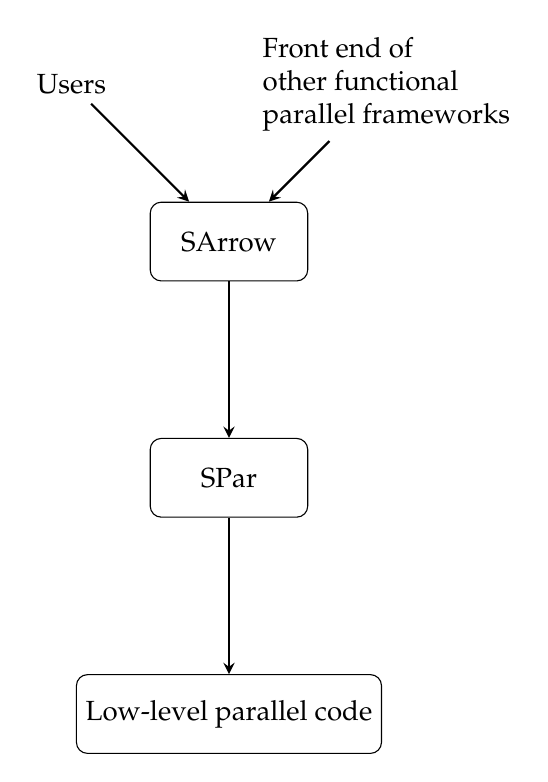
\begin{tikzpicture}[xscale=.5]
    \tikzstyle{proc}  = [rectangle, rounded corners, minimum width=2cm, minimum height=1cm,text centered, draw=black] 
    \tikzstyle{proc1} = [circle,  minimum width=1cm, minimum height=1cm,text centered, draw=black] 
    \tikzstyle{arrow} = [thick,->,>=stealth]
    \node (a) [proc] at (0, 3)  {SArrow};
    \node (b) [proc] at (0, 0)  {SPar};
    \node (c) [proc] at (0, -3) {Low-level parallel code};
    \node (d)  at (-4, 5) {Users};
    \node (e) [align=left] at (4, 5) {Front end of \\ other functional  \\ parallel frameworks};
    \draw[arrow] (a) to (b);
    \draw[arrow] (b) to (c);
    \draw[arrow] (d) to (a);
    \draw[arrow] (e) to (a);
    \end{tikzpicture}
    \caption{Visualization of the workflow}
    \label{intro:fig:workflow}
\end{figure}
The result of project is a embedded high-level framework in Haskell that is capable of generating low-level parallel code. The major contributions are:
\begin{enumerate}
    \item \textbf{Session-typed intermediate language. } We create an intermediate embedded domain specific language (EDSL): SPar: a session typed free monad EDSL for message passing concurrency. This language can be typed by local types, and hence, we can apply multiple results from the multiparty session types to our framework, especially in terms of safety of generated code and reasoning of communication patterns.
    \item \textbf{Intuitive user interface. } One innovation of this project is that we apply the mature Arrow interface for users to express parallel computations. We call the interface SArrow: an arrow interface for writing SPar expressions. It is an abstraction layer on top of SPar, which hides communication primitives from users so that users can express parallel algorithms similar to what they would write for sequential programs.
    \item \textbf{Multiple backends. } We create a backend to generate parallel C code from SPar expressions. The core of the backend is Instr: a low-level EDSL that is independent of target languages. This means that we can support multiple target languages with ease without re-implementing multiple backends. In addition to the code generation backend, we implement an interpreter backend in Haskell for experimenting and fast verification.
    \item \textbf{Evaluations. } Finally, we show the expressive power of the framework by implementing several common computation patterns and three algorithms using our interface. We evaluate the performance of the generated code from the algorithms on high-performance computers as well as PCs. 
\end{enumerate}
The \figref{intro:fig:workflow} summaries the workflow of the framework visually. The main principle supporting the framework is that we convert data flow into communications and from the communication patterns, we gain parallel codes. The results of expressing computation in the framework are 1) compilation to efficient deadlock-free low-level parallel programs and 2) a set of local types to reason the structure of the parallel computation.

At the end of the project, we have discovered two use case of the framework. The primary application is a stand-alone tool to generate parallel C code, and another is a backend for other data-flow based parallel frameworks. 

\section{Report outlines}

\charef{chap:b} gives an overview of the background and related researches. We present the syntax and semantics of SPar in \charef{chap:spar} followed by \charef{chap:impl} introducing the implementation aspect of SPar like session typing and interpreter. \charef{chap:arrow} demonstrates the Arrow interface with examples of parallel patterns formed by the interface and justification of the interface satisfying arrow laws. The discussion about some implementation specific issues like role allocation is also contained in \charef{chap:arrow}. In \charef{chap:cg}, we show the code generation backend and discuss our solutions to challenges when compiling to C, i.e. the problem of representing polymorphic algebraic data structure in C. \charef{chap:eval} explains our benchmarks and shows the performance of the generated code. This chapter can also be regarded as a tutorial on how to use the framework. Finally, we conclude with potential future improvements and remarks on this project. We also include the generated C code in the appendix for curious readers.
\chapter{Background} \label{b}
% This section is an overview of arrows, multiparty session types (MPST) and free monad. Arrow is an interface of implicit data flow, and MPST can be used to describe explicit data flow. Free monad is a technique to convert normal DSL to a monadic DSL. 
% As mentioned in the \secref{i:m}, this section is an overview of a high-level language (\secref{b:arrows} and \secref{b:pal}), from which a translation rule will be proposed to our intermediate languages, multiparty session types (\secref{b:mpst}), the theoretical backbone giving rich features of the intermediate languages, and the free monad (\secref{b:fm}), a technique in designing the intermediate languages.
This section is an overview of techniques that influence the design choices of our monadic language for parallel computation. First of all, we give an overview of techniques applied in the high-level parallel programming framework: arrows (\secref{b:arrows}) and recursion schemes (\secref{b:rs}). We then introduce several techniques for message-passing concurrency: multiparty session types (\secref{b:mpst}) and monadic languages for concurrency (\secref{b:mo}). In the end, we introduce free monads (\secref{b:fm}), a technique valuable in implementing embedded domain-specific languages (EDSL).

\section{Arrows} \label{b:arrows}
Arrow is a general interface to describe computation. It can ease the process of writing structured code suitable for parallelising. It also demos a common feature of the frameworks: parallelizability is empowered by underlying implicit but precise data-flow. On the other hand, converting to low-level message-passing code, which requires programmers to define communication using message-passing function and primitives, makes the data-flow explicit.
\subsection{Definition}
\coref{b:ar:c1} shows the Arrow definition in Haskell. Intuitively, an arrow type \hask{y a b}(that is, the application of the parameterised type \hask{y} to the two parameter types \hask{b} and \hask{c}) can be regarded as a computation with input of type \hask{b} and output of type \hask{b}\cite{hughesGeneralisingMonadsArrows2000}. Visually, arrows are like pipelines (shown in \figref{b:ar:p1}). In Haskell, an arrow \hask{y} is a type that implements the following interface (type classes in Haskell are roughly interfaces). \hask{arr} converts an arbitrary function into an arrow. \hask{>>>} sequences two arrows (illustrated in \figref{b:ar:seq}). Taking two input,  \hask{first} apply the arrow to the first input while keeping the second untouched (\figref{b:ar:first}). Conversely, \hask{second} modifies the second input and keeps the first one unchanged. \hask{***} applies two arrows to two input side by side (\figref{b:ar:par}). \hask{&&&} takes one input and applies two separate arrows to the input and its duplications (\figref{b:ar:dup}).
% TODO add reference to arrow visualization

The simplest instance of arrow class is the function type (shown in \coref{b:ar:c2}). It is worth noticing that only \hask{arr} and \hask{***} need to be implemented. The reset of function in the arrow type class can be defined in terms of the two functions. For example, \mintinline{text}{f &&& g = (f *** g) . arr (\b -> (b, b))} and \mintinline{text}{first = (*** id)}
\begin{code}
  % \inputminted{haskell}{background/ar-def.hs}
  \begin{minted}{haskell}
    class Arrow y where 
      arr :: (a -> b) -> y a b
      first :: y a b -> y (a, c) (b, c)
      second :: y a b -> y (c, a) (c, b)
      (***) :: y a c -> y b d -> y (a, b) (c, d)
      (&&&) :: y a b -> y a c -> y a (b, c)
  \end{minted}
  \caption{Arrow class in Haskell}
  % \ccaption{Arrow class in Haskell}{
    % \begin{itemize}
      % \item[\cref{ar-def:1}] Types of arrow functions 
    % \end{itemize}
  % }
  \label{b:ar:c1}
\end{code}
\begin{code}
  % \inputminted{haskell}{background/ar-func.hs}
  \begin{minted}{haskell}
    instance Arrow (->) where
      arr f = f
      (***) f g ~(x,y) = (f x, g y)
  \end{minted}
  \caption{$(\rightarrow)$ instance of Arrow class}
  \label{b:ar:c2}
\end{code}
\begin{figure*}
  \centering
  \begin{subfigure}[b]{0.475\textwidth}
      \centering
      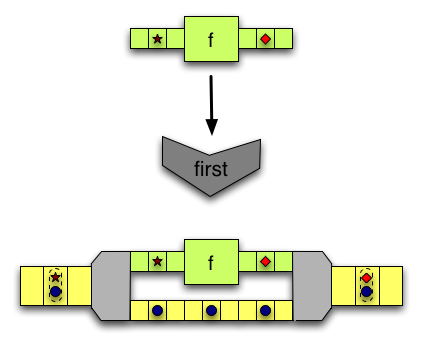
\includegraphics[width=\textwidth]{background/image/ArrowsConveyors_first2.png}
      \caption{\hask{first}}
      \label{b:ar:first}
  \end{subfigure}
  \hfill
  \begin{subfigure}[b]{0.475\textwidth}  
      \centering 
      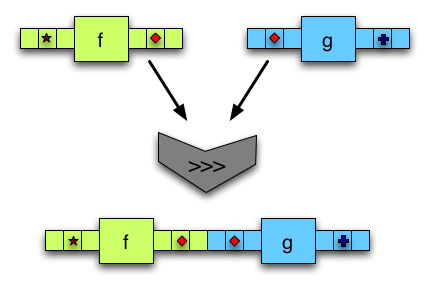
\includegraphics[width=\textwidth]{background/image/ArrowsConveyors_bind2.png}
      \caption{\hask{>>>}}
      \label{b:ar:seq}
  \end{subfigure}
  \vskip\baselineskip
  \begin{subfigure}[b]{0.475\textwidth}   
      \centering 
      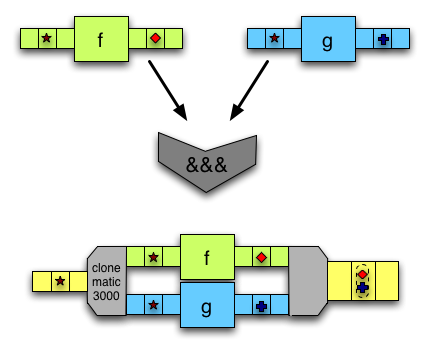
\includegraphics[width=\textwidth]{background/image/ArrowsConveyors_ampersand2.png}
      \caption{\hask{&&&}}
      \label{b:ar:dup}
  \end{subfigure}
  \quad
  \begin{subfigure}[b]{0.475\textwidth}   
      \centering 
      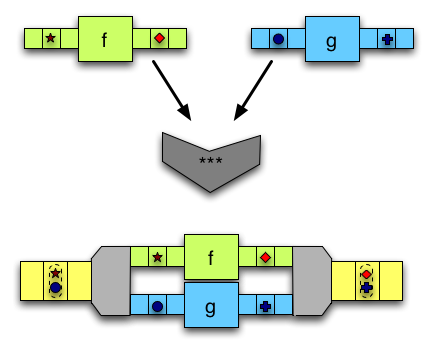
\includegraphics[width=\textwidth]{background/image/ArrowsConveyors_star2.png}
      \caption{\hask{***}}
      \label{b:ar:par}
  \end{subfigure}
  \caption
  {\small The visual representations of arrow combinators\cite{HaskellUnderstandingArrows}}
  \label{b:ar:p1}
\end{figure*}
\subsection{Example: Calculate the mean}
Consider the a function to calculate the mean from a list of floating number, we will compare the usual, arrows implementations. Implementation using arrows can be regarded as point-free programming. Point-free programming is programming paradigm where function definitions only involve combinators and function composition without mentioning variables\cite{TacitProgramming2019}. 

\begin{minted}{haskell}
mean :: [Float] -> Float
mean xs = sum xs / (fromIntegral . length) xs

mean' :: [Float] -> Float
mean' = (sum &&& (length >>> fromIntegral)) >>> uncurry (/)
\end{minted}
The arrows implementation can be visualised in \figref{b:ar:p2}.
\begin{figure}[!ht]
  \centering
  % \includegraphics[width=8cm]{example-image} 
  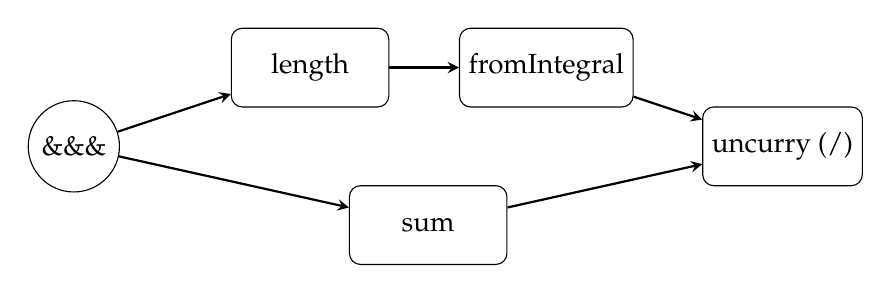
\begin{tikzpicture}[xscale=1.5]
    \tikzstyle{proc} = [rectangle, rounded corners, minimum width=2cm, minimum height=1cm,text centered, draw=black] 
    \tikzstyle{proc1} = [circle,  minimum width=1cm, minimum height=1cm,text centered, draw=black] 
    \tikzstyle{arrow} = [thick,->,>=stealth]
    \node (a) [proc1] at (0, 0) {\&\&\&};
    \node (b) [proc] at (2, 1) {length};
    \node (c) [proc] at (4, 1) {fromIntegral};
    \node (d) [proc] at (6, 0) {uncurry (/)};
    \node (e) [proc] at (3, -1) {sum};
    \draw[arrow] (a) to (b);
    \draw[arrow] (b) to (c);
    \draw[arrow] (c) to (d);
    \draw[arrow] (a) to (e);
    \draw[arrow] (e) to (d);
  \end{tikzpicture}
  \caption{Visualization of mean'}\label{b:ar:p2}
\end{figure}
\begin{minted}{haskell}
mean'' :: [Float] -> Float
mean'' = liftM2 (/) sum (fromIntegral . length)
\end{minted}
Arrows are not the only way to form point-free programs. The above code snippet is the more traditional approach form of point-free mean function in Haskell. We can argue this form of point-free function is more difficult to understand compared to arrows because it involves knowledge of monads (\hask{liftM2}) and does not map to intuitive data-flow.

The simple example demos that arrows combinators make writing point-free programs easier. Arrows union the implementation of algorithm and data-flow in the algorithm. 

\subsection{Application in parallel computation}
From the previous example, the data flow of programs written regarding arrow combinators can be easily visualised (shown in \figref{b:ar:p1}). It is intuitive to recognise that the clean separation between the flow of data and actual computation will be useful in generating parallel code. Indeed, arrow describes data flow implicitly, and it is an example of the so-called algebraic pattern. Many works \cite{braunArrowsParallelComputation2018, elliottGenericFunctionalParallel2017b, AlgebraicMultipartyProtocol} has been done to generate parallel code from algebraic patterns.
In particular, details of \cite{AlgebraicMultipartyProtocol} are introduced in later section. % TODO

\section{Recursion Schemes} \label{b:rs}
Recursion schemes are patterns for expressing general computation. In particular, they are like high order function abstracting recursion so that programmer can express any kind of recursion by data structures combined with recursion schemes instead of writing explicit recursive functions.
\subsection{Definition}
We will introduce three typical recursion schemes: catamorphisms, anamorphisms and hylomorphisms (seen in \coref{p:pal:c3}). As mentioned before, recursion schemes express recursion with the help of data structures, in particular, the fixed point of data structures (seen in \coref{p:pal:c2})
\begin{code}
\begin{minted}{haskell}
newtype Fix f = Fix { unfix :: f (Fix f) }

data TreeF a =
    Node a a
  | Leaf int
  | Empty
  deriving Functor

type Tree = Fix TreeF
\end{minted}
\caption{Definition of fix point of data structures} \label{p:pal:c2}
\end{code}

Anamorphisms takes a function from a to f a (called the co-algebra) and a value a and return the Fix f. Used Tree as an example, anamorphisms takes a single value a and applies the co-algebra to the value. It continues to apply itself to the branches of the TreeF recursively and finally expands a single value to a complete tree. Intuitively, anamorphism unfolds a single value to a complicated data structure top-down.

Catamorphisms is the reverse of anamorphisms, folding a data structure to a single value bottom-up. It takes a function from f a to a (called the algebra) and Fix f to fold and return a single value a. Catamorphisms and anamorphisms describe the process globally (from a to Fix f and from Fix f to a) while co-algebra and algebra capture what happened locally. The elegant part is while co-algebra and algebra do not involve with any recursion data structure (TreeF is not recursive), catamorphisms consumes recursive data structure while anamorphism builds them.

Hylomorphisms applies anamorphism followed by catamorphisms. It is the most common pattern to use. We will use an example to illustrate its usefulness. It can be thought of as an abstract divide and conquer algorithm.
% TODO add Divided and conquer analogy
\begin{code}
\begin{minted}{haskell}
ana :: Functor f => (a -> f a) -> a -> Fix f
ana coalg = Fix . fmap (ana coalg) . coalg

cata :: Functor f => (f a -> a) -> Fix f -> a
cata alg = alg . fmap (cata alg) . unfix

hylo :: (f b -> b) -> (a -> f a) -> b -> a 
hylo g f = f . fmap (hylo f g) . g
\end{minted}
\caption{Recursion schemes in haskell} \label{p:pal:c3}
\end{code}

\subsection{Example: Merge sort} \label{b:rs:ex}
We can write merge sort recursively. First of all, we split the list in half and then apply the merge sort recursively to both parts and finally we merge two lists into a single list. 

To write merge sort in terms of recursion scheme, we need to define the recursive structure to represent the control structure. By the definition of merge sort, this structure must have a case with two branches, a base case representing a singleton list and a base case representing an empty list hence this structure is the TreeF we defined above. Splitting a list is like co-algebra while merging is like algebra. We use hylomorphisms to combine them hence getting a sorted list (seen in \coref{p:pal:c4}).
\begin{code}
\inputminted{haskell}{project/pal-ms.hs}
\caption{Merge sort using hylomorphisms} \label{p:pal:c4}
\end{code}
\section{Multiparty session types} \label{b:mpst}
In complicated distributed systems, participants agree on a protocol, specifying type and direction of data exchanged. Multiparty session types are a branch of behavioural types specifically targeted at describing protocols in distributed systems based on asynchronous communication \cite{coppoGentleIntroductionMultiparty2015}. They are a type formalism used to model communication-based programming by codifying the structure of communication. The evolution of computing from the era of data processing to the era of communication witnessed the growth and significance of the theory of session types.

The theory of multiparty session type contains three main elements. Global types (seen in \secref{b:mpst:st}), local (session) types and processes. Processes are the concrete descriptions of the behaviour of the peers involved in the distributed system \cite{coppoGentleIntroductionMultiparty2015} using a formal language. Usually, the most used and the original language is $\pi$-calculus \cite{milnerCalculusMobileProcesses1992}.  However, for the simplicity, we will not introduce $\pi$-calculus % and use message passing primitives in Haskell (seen in section \label{b:mo:mpc}) instead. 
The coming sections are an intuitive introduction of session types by examples.
% TODO: Add descriptions about the MPST 1. describes explicit dataflow 2. so it can be used as the high-level programming languages to generate parallel code 3. in \secref{b:mpst:app}.
\subsection{Global types and local types} \label{b:mpst:st}
Global type is at the most abstract level, describing a communication protocol from a neutral viewpoint between two or more participants\cite{coppoGentleIntroductionMultiparty2015}. The syntax of the global types is shown in \tabref{b:mpst:gt} and an example of global types is shown in \tabref{b:mpst:gtex}.

Local types or session types characterise the same communication protocol as the global type, but from the viewpoint of each peer \cite{coppoGentleIntroductionMultiparty2015}. Each process is typed by local type. The syntax of local types is shown in \tabref{b:mpst:lt} and an example of local type is shown in \tabref{b:mpst:ltex}. 

The relationship between global types and local types are established by the projection operator (seen in the \secref{b:mpst:proj}), and a type system performs syntactic checks, ensuring that processes are typed by their corresponding local types. Hence, at the compile time, three important properties follow \cite{coppoGentleIntroductionMultiparty2015}. 
\begin{itemize}
  \item \textbf{communication safety}: Mismatches between the types of sent and expected messages, despite the same communication channel is used for exchanging messages of different types, do not exist \cite{coppoGentleIntroductionMultiparty2015}. 
  \item \textbf{protocol fidelity}: The interactions that occur are accounted for by the global type and therefore are allowed by the protocol \cite{coppoGentleIntroductionMultiparty2015}.
  \item \textbf{progress}: Every message sent is eventually received, and every process waiting for a message eventually receives one \cite{coppoGentleIntroductionMultiparty2015}.
\end{itemize}
We will learn that these properties are valuable not only in the distributed system but also in the domain of parallel computing in \secref{b:mpst:app}.
% In the theory of multiparty session types, the whole distributed system is described by global types representing the communication protocols from a global viewpoint.  Each process is typed by local types which characterise the same communication protocols as global types but from a perspective of individual participants \cite{coppoGentleIntroductionMultiparty2015}.
\begin{table}[ht]
\centering
\begin{grammar}{G\Coloneqq}{Global types}
  p \rightarrow q : \langle S \rangle.G & Value exchange \\
  p \rightarrow q : \langle T \rangle.G & Channel exchange \\
  p \rightarrow q : \{ l_i : G_i \}_{i \in I} & Bracnhing \\
  \mu \mathbf{t}.G  \mid \mathbf{t} \mid \text{end} & Recursion/End
\end{grammar}
\caption{Global types} \label{b:mpst:gt}
\end{table}
\begin{table}[ht]
\begin{grammar}{S\Coloneqq}{Sorts}
  \text{bool} \mid \text{nat} \mid \text{string} \\
  \dots\\
\end{grammar}
\hfill
\begin{grammar}{T\Coloneqq}{Session types/local types}
  ! \langle p, S \rangle . T & Send value\\
  ! \langle p, T \rangle . T & Send channel\\
  ? ( p, T ) . T & Channel Receive\\
  ? ( p, S ) . T & Sorts Receive\\
  \oplus \langle p, \{ l_i : T_i \}_{i \in I} \rangle & Selection \\
  \&(p, \{l_i : T_i \}_{i \in I}) & Bracnhing \\
  \mu \mathbf{t}.T  \mid \mathbf{t} \mid \text{end} & Recursion/End
\end{grammar}
\caption{Session types/local types} \label{b:mpst:lt}
\end{table}
\begin{table}[ht]
  \begin{minipage}{0.45\textwidth}
    \begin{enumerate}
      \item Customer(0) sends an order number to Agency(1), and Agency sends back a quote to the customer.
      \item If Customer is happy with the price then Customer selects accept option and notifies Agency.
      \item If Customer thinks the price is too high then Customer terminate the trade by selecting reject.
      \item If accept is selected, Agency notify both Customer and Agency2(2). 
      \item Customer sends an address to Agency2 and Agency2 sends back a delivery date.
    \end{enumerate}
  \end{minipage}
  \hfill
  \begin{minipage}{0.45\textwidth}
    \begin{align*}
      G = \\
      & 0 \rightarrow 1: && \langle \text{string} \rangle .\\
      & 1 \rightarrow 0: && \langle \text{int} \rangle .\\
      & 0 \rightarrow 1: \{ && \text{accept}: \\
      & && 1 \rightarrow \{ 0, 2 \}: \langle \text{string} \rangle . \\
      & &&  0 \rightarrow 2: \langle \text{string} \rangle .\\
      & &&  2 \rightarrow 0: \langle \text{int} \rangle . \text{end}, \\
      & && \text{reject}: \text{end} \} \\
    \end{align*}
  \end{minipage}
  \caption{An example of a protocal described by global types G}
  \label{b:mpst:gtex}
\end{table}
\begin{table}[ht]
  \begin{minipage}{0.45\textwidth}
    \begin{align*}
      S \triangleq \mu t.(\&\{ & \text{balance}: ![\text{nat}];t, \\
        & \text{deposit}: ?[\text{nat}];![\text{nat}];t, \\
        & \text{exit}: \text{end}\}) \\
    \end{align*}
  \end{minipage}
  \hfill
  \begin{minipage}{0.45\textwidth}
    \begin{align*}
      C \triangleq \oplus \{ &\text{balance}: ?[\text{nat}];\text{end}, \\
                             &\text{deposit}: ![\text{nat}];?[\text{nat}];\text{end} \} 
    \end{align*}
  \end{minipage}
  \caption{Session types of client and server end point of a ATM service}
  \label{b:mpst:ltex}
\end{table}
\subsubsection{Projection between global types and local types} \label{b:mpst:proj}
Projection is the formalisation of the relationship between global and local types. It is an operation extracting the local type of each peer from the global type \cite{coppoGentleIntroductionMultiparty2015}. The definition of projection is shown in \tabref{b:mpst:pdef}.

As an example, a projection of global type in \tabref{b:mpst:gtex} is
$$
  G \upharpoonright 0 = !\langle 1, \text{string} \rangle;?(1, \text{string});\&(1, \{ \text{accept}: ?(1, \text{string});!\langle 2, \text{string} \rangle;?(2, \text{int}), 
  \text{reject}: \text{end} \})
$$  
\begin{table}[H]
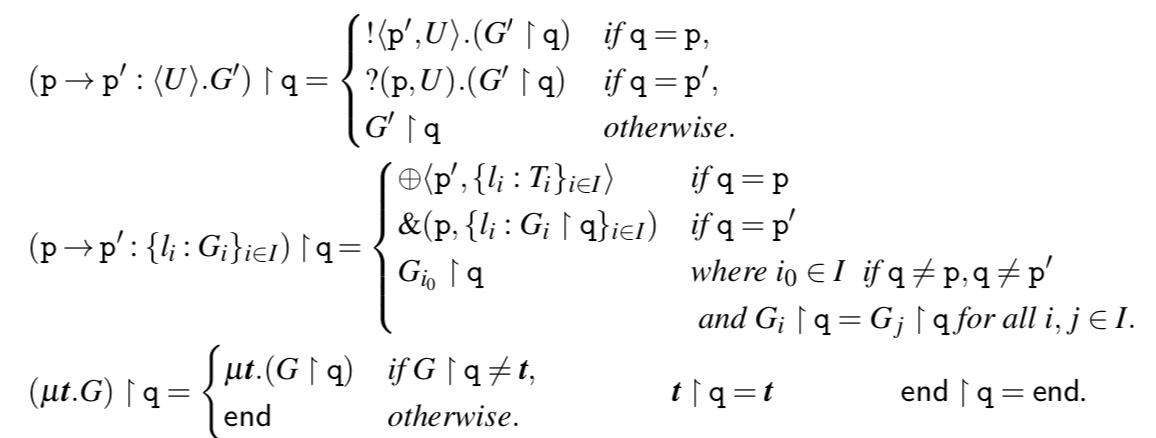
\includegraphics[width=\textwidth]{background/image/proj-def.png}
\caption{The definition of projection of a global type G onto a participants q\cite{coppoGentleIntroductionMultiparty2015}}
\label{b:mpst:pdef}
\end{table}
\subsubsection{Duality of session types}
In binary session types where all protocals are pairwise, duality formalises the relationship between the types of opposite endpoints. For a type $T$, its dual or co type, written $\bar{T}$ is defined inductively as in \tabref{b:mpst:dualdef}.
\begin{table}[H]
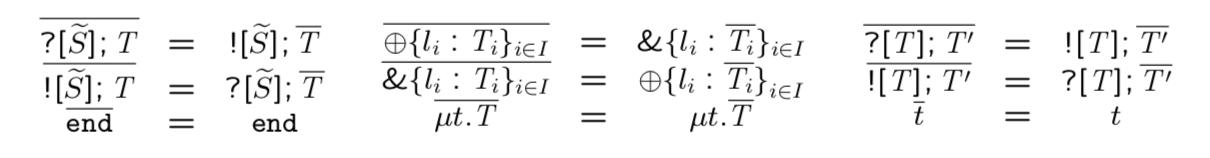
\includegraphics[width=\textwidth]{background/image/dual-def.png}
\caption{Inductive definition of duality}
\label{b:mpst:dualdef}
\end{table}

Duality is essential for checking type compatibility. Compatible types mean that each common channel $k$ is associated with complementary behaviour: this ensures that the interactions on $k$ run without errors. 

In order to apply duality into multiparty session types in which more than two participants are allowed, the partial projection operation (seen in \cite{coppoGentleIntroductionMultiparty2015}) from multiparty session type to binary session type was introduced to allow reusing the definition of duality after applying the partial projection.
% \begin{table}[H]
% \caption{The pa}
% \label{b:mpst:partproj}
% \end{table}
% \begin{table}[ht]
% \begin{align*}
% \end{align*}
% \caption{Inductive definition of duality} \label{b:mpst:dual}
% \end{table}
% \subsection{Example: arithmetic server}
\subsection{Applications in parallel computing} \label{b:mpst:app}
Multiparty session types not only have rich applications in distributed systems but also value in the domain of parallel computation. 

Existing work\cite{ngSafeMPICode} has shown how to generate MPI\footnote{Message Passing Interface (MPI) is a standardised and portable message-passing standard designed by a group of researchers from academia and industry to function on a wide variety of parallel computing architectures \cite{MessagePassingInterface2018}.} programs using session types. Users describe the communication topology as a skeleton using a protocol language which is type checked by session types. After that, an MPI program is generated by merging the skeleton and user-provided kernels for each peer. The parallel code obtained in this way is guaranteed to be deadlock-free and progressing. 

\section{Message passing concurrency} \label{b:mo}
This section introduces some interfaces for message passing concurrency from the primitive case: channel to more advanced one: monad for message passing concurrency.

For simplicity, they are represented in Haskell, but in general, most languages can implement similar interfaces. 
\subsection{Primitives for message-passing concurrency} \label{b:mo:mpc}
In \secref{b:mpst}, channels are bi-directional and used for communication between two parties. In Haskell, channel primitives are represented in \coref{b:mo:c1}. However, just using these primitives cannot guarantee progress or communication safety. For example, a program that has one thread writing channel once combined with another thread reading channel twice is type-correct but will cause deadlock. Many kinds of research to encode MPST using Haskell's type system are presented in \cite{orchardSessionTypesLinearity} so that an (MPST) type-correct Haskell program assures progress, communication safety and session fidelity.
\begin{listing}[ht]
  \inputminted{haskell}{background/mo-chan.hs}
  \caption{Channel primitives in Haskell}
  \label{b:mo:c1}
\end{listing}
\subsection{Concurrency Monads}
The work done by \cite{claessenFunctionalPearlsPoor1999} constructs a monad to express concurrent computation. The definition is in \coref{b:mo:def}. \hask{Action} is the algebraic datatype representing basic concurrency primitives. \hask{Atom}, the atomic unit of computation, is a computation (wrapped in the \hask{IO} monad) followed by an action. \hask{Fork} is two parallel action. \hask{Stop} is the termination of an action. type \hask{C} is a special case of the continuation monad. The continuation monad is an encapsulation of computations in continuation-passing style (CPS)\footnote{In continuation-passing style function result is not returned, but instead is passed to another function, received as a parameter (continuation)\cite{ControlMonadCont}}. SO \hask{C a} is a CPS computation that produces an intermediate result of type \hask{a} within a CPS computation whose final result type is \hask{Action}. With the help of the monad \hask{C}, sequencing and composing actions can use monadic bind.
\begin{code}
  \begin{minted}{haskell}
data Action =
    Atom (IO Action)
  | Fork Action Action
  | Stop

newtype C a = C { runC :: (a -> Action) -> Action } #\clabel{mo-cm:5}#
    
instance Monad C where
    (>>=) :: C a -> (a -> C b) -> C b #\clabel{mo-cm:6}#
    m >>= f  = C $ \k -> runC m (\v -> runC (f v) k)
    return :: a -> C a
    return x = C $ \k -> k x
  \end{minted}
  \caption{The definition of concurrency monad}
  \label{b:mo:def}
\end{code}


The idea is using continuation to represent the "future" so that computation can pause and resume as well as expressing sequential computation. Atom wraps the actual computation and Fork is responsible for spawning threads. In addition, in order to write programmes in a monadic way easier, some helper functions are defined (shown in \coref{b:mo:helper}). \hask{atom} lifts an IO computation to \hask{C}. And \hask{fork} takes a computation in \hask{C} and return a \hask{C} which involves the \hask{Fork} action. Given a \hask{C a}, \hask{action} gives the result of running the CPS computation. We use \hask{\_. Stop} to represent the final continuation (\hask{Stop} action is the last action). 
\begin{code}
\begin{minted}{haskell}
atom :: IO a -> C a
atom m = C $ \k -> Atom $ do
    r <- m
    return $ k r

fork :: C () -> C ()
fork m = C $ \k -> Fork (runC m (const Stop)) (k ())

action :: C a -> Action
action m = m (\_. Stop)
\end{minted}
\caption{Helper functions}
\label{b:mo:helper}
\end{code}
An example of programme written in the concurrency monad is shown below.
\begin{code}
  \begin{minted}{haskell}
example :: C ()
example = do 
  atom $ putStrLn "Hello" 
  name <- atom getLine 
  fork $ atom $ putStrLn "World"
  atom $ putStrLn name
  \end{minted}
\end{code}
We can easily define a round-robin scheduler for programmes in this monad. We can regard a list of action as a queue of threads that are running concurrently. \hask{schedule} will pattern match on the head of the list. If it is \hask{Atom} then the scheduler will run the computation (seen \hask{a <- ioa} at \cref{mo-cm:1}) and pause its remaining computation and put it at the end of the thread queue (seen at \cref{mo-cm:2}). If it is \hask{Fork} then the scheduler will spawn the thread and put the new thread and the current thread to the bottom of the queue (seen at \cref{mo-cm:3}). Finally, If it is \hask{Stop} then it means this thread has finished and the scheduler will resume with the rest of threads in the queue. For example, to run the above example, we call \hask{schedule [action example]}.
\begin{code}
  \begin{minted}{haskell}
schedule :: [Action] -> IO () 
schedule [] = return ()
schedule (a:as) = sched as a
    
sched :: [Action] -> Action -> IO ()
sched as (Atom ioa) = do
    a <- ioa #\clabel{mo-cm:1}#
    schedule $ as ++ [a] #\clabel{mo-cm:2}#
sched as (Fork a1 a2) = schedule $ as ++ [a2, a1] #\clabel{mo-cm:3}#
sched as Stop = schedule as
  \end{minted}
\end{code}

The concurrency monad can be extended to support many features. For example, work done by \cite{marlowMonadDeterministicParallelism} modifies the definition of Action as well as implements a work-stealing parallel scheduler (seen in \coref{b:mo:c3}) to build a monad for parallel computation. 

Besides, extending the concurrency monad to monad for message-passing concurrency can be done by adding channel primitives like newChan, writeChan and readChan into the Action. Since channel primitives are possible to represent in this monad, we naturally think of its prospect in connecting with MPST (will be discussed in the later section).
\begin{code}
  % \inputminted{haskell}{background/mo-par.hs}
  \begin{minted}{haskell}
newtype IVar a = IVar (IORef (IVarContents a)) #\clabel{po:ivar}#
data IVarContents a = Full a | Blocked [a -> Action.]
    
data Action .=
    Fork Action Action
  | Stop
  | forall a . Get (IVar a) (a -> Action) #\clabel{po:get}#
  | forall a . Put (IVar a) a Action #\clabel{po:put}#
  | forall a . New (IVar a -> Action)
  \end{minted}
  \ccaption{Par Monad}{
    \begin{itemize}
      \item[\cref{po:ivar}] Parent threads and child threads communicate data via IVar
      \item[\cref{po:get}] Get operation blocks when the underlying IVarContents is Blocked  
      \item[\cref{po:put}] Put operation updates the underlying IVarContetns to Full with the result a and resume the list of blocking threads by applying a to the continuation.
    \end{itemize}
  }
  \label{b:mo:c3}
\end{code}

In summary, many techniques and ideas like continuation presented in the implementation of this monad afford us inspirations in designing our intermediate language.
\section{Free monad} \label{b:fm}
% TODO add reference to the concurrency monad, show that monad C is not necessary
Free monad\cite{contributorsCatsFreeMonads} is a concept from category theory. Intuitively, a free monad as a programming abstraction is a technique for implementing EDSLs, where a functor represents basic actions of the EDSL and the free monad of this Functor provides a way to sequence and compose actions. Speaking of the advantages, we are particularly interested in its benefits in flexible interpretations which will be illustrated by an example (\secref{b:fm:e}) and discussed further (\secref{b:fm:a}).
\subsection{Definition}
In practice, a free monad in Haskell can be defined as an algebraic data type(ADT) (shown in \coref{b:fm:c1}). \hask{Free f} is the monad produced given a functor \hask{f}. \hask{Free} has two type constructors: \hask{Pure} and \hask{Free}. \hask{Monad (Free f)} is the Haskell implementation of the Monad interface for \hask{Free f}. Many useful helper functions are derived from the simple definition of the free monad (shown in \coref{b:fm:c2}). \hask{liftF} lift the functor to its free monad representations. \hask{freeM} maps a natural transformation of functor (\hask{f a -> g a}) to the natural transformation of their free monad versions. Given \hask{m} is a monad, \hask{freeM} is a special case of interpreting \hask{Free m a}: to the \hask{m} monad itself. Finally, \hask{interpret} shows the power of free monad. We can interpret the free monad version of a functor \hask{f} to any monad \hask{m} given a natural transformation from \hask{f} to \hask{m}.
\begin{code}
  \inputminted{haskell}{background/fm-construction.hs}
  \caption{Free monad in Haskell}
  \label{b:fm:c1}
\end{code}
\begin{code}
  \inputminted{haskell}{background/fm-helper.hs}
  \caption{Helper functions based on free monad}
  \label{b:fm:c2}
\end{code}
\subsection{Example} \label{b:fm:e}
Free monad is useful in interpreting an abstract syntax tree (AST). In order to apply free monad to a given AST, we can follow a routine \cite{contributorsCatsFreeMonads}.
\begin{enumerate}
  \item Create an AST, usually represented as an ADT
  \item Implement functor for the ADT
  \item Create helper constructors to Free ADT for each type constructor in ADT by liftF 
  \item Write a monadic program using helper constructors. It is essentially a program written in DSL operations.
  \item Build interpreters for Free ADT by interpreting
  \item Interpret the program by the interpreter.
\end{enumerate}
We will demo the above procedure by a made-up example. We would like to build a simple EDSL for getting customers' name and greeting customers. First of all, we build a functor \hask{GreetingF} to represent the basic operations: getting the name and greeting. Then we wrap the functor with \hask{Free} constructor so that a program written in our EDSL can be regarded as a Haskell expression with type \hask{Free GreetingF a}.
\begin{code}
\begin{minted}{haskell}
data GreetingF next
  = Getname (String -> next)
  | Greet String next
  deriving Functor

type Greeting = Free GreetingF
\end{minted}
% \caption[.]{
%   \begin{minipage}{\linewidth}
%     Par monad
%     \begin{itemize}
%       \item[\cref{mylin2} :] hello 
%       \item[\cref{mylin2} :] hello 
%     \end{itemize}
%  \end{minipage}
%  }
\end{code}
Then we create helper functions of Greeting using liftF.
\begin{minted}{haskell}
getName = liftF $ Getname id
greet str = liftF $ Greet str ()
\end{minted}
Then we can write a simple program using operations provided by Greeting.
\begin{minted}{haskell}
exampleProgram :: Greeting ()
exampleProgram = do
    a <- getName
    greet a
    b <- getName
    greet b
\end{minted}
Then we can easily implement an interpreter for the example program
\begin{minted}{haskell}
goodMorningInterpreter :: Greeting a -> IO a
goodMorningInterpreter = interpret helper
    where
        helper (Getname next) = fmap next getLine
        helper (Greet str next) = putStrLn ("Good morning " ++ str) >> return next  
\end{minted} 
Finally, execute the program.
\begin{minted}{bash}
ghci:> goodMorningInterpreter examplePrograe
Tom
Good morning Tom
Mary
Good morning Mary
\end{minted}
% \begin{listing}
%   \inputminted{haskell}{background/fm-example.hs}
%   \caption{An example of free moand}
%   \label{b:fm:c3}
% \end{code}

\subsection{Applications} \label{b:fm:a}
As illustrated by the example (\secref{b:fm:e}), free monad decouple the abstract syntax tree of domain specific language (DSL) and the interpreter. Interpreters with different purposes can be implemented without changing the syntax.

In the project, we apply free monad to the intermediate language so not only we make the languages monadic for free but also benefits from decoupling the interpreter and the syntax to implement different interpreters, e.g. Simulator, code generators to different platforms easily.
% % \chapter{Design and Implementation}
\chapter{TBD:the theory and the practice}
\section{Parallel algebraic language} \label{b:pal}
Parallel algebraic language (PAL) is an example of the high-level languages to generate parallel code, proposed in the paper \cite{authorAlgebraicMultipartyProtocol2018}. In this project, a translation rule from this languages to the intermediate languages will be introduced.
\subsection{Syntax}
Besides primitives type like int, unit and function types, PAL use four functors to form more types hence representing complicated data structures by composing them (seen in table). For example, a list of integer is expressed in \coref{p:pal:c1}.
\begin{table}[ht]
\begin{grammar}{F_1, F_2 \Coloneqq}{}
    I & Identity functor\\
    K t & Constatnt functor\\
    F_1 + F_2 & Sum functor\\
    F_1 \times F_2 & Product functor
\end{grammar}
\hfill
\begin{grammar}{t_1, t_2 \Coloneqq}{Type}
    () \mid \text{int} \mid \dots & Primitive types\\
    F \ t_1 & Functor types\\
    \mu .F & Recursive types\\
\end{grammar}
\caption{Functor and Type definitions}
\end{table}
\begin{code}
\begin{lstlisting}{language=Haskell}
    newtype L = K () + K Int * I
    type List = Rec L
\end{lstlisting}
\caption{Type of integer list in PAL}
\label{p:pal:c1}
\end{code}

An important feature of PAL is the lack of usual control flow like if branch or while loop, instead, it uses data structures to replace control flow. Data structures in PAL not only store data but also serves as control structures. It uses the idea of recursion schemes (seen in \secref{b:rs}) to build sophiscated algorithms. 

To summary, algorithms in PAL are represented as a series of transformations of data, making it easy to transform the PAL programmes to programmes in arrows mechanically since arrows also express flow of data and their transformations naturally. This property allows us to generate parallel code without burnders.

\subsection{Example: Merge sort}

Like the merge sort example in \secref{b:rs:ex}, PAL make these recursion shcemes built-in and hence express computation. A merge sort in PAL is shown in \coref{p:pal:c5}
\begin{code}
\begin{lstlisting}[language=haskell]
poly T = K (() + int) + I * I;
poly L = K () + K int * I;

atom split : Rec L -> T Rec L;

atom merge : T Rec L -> Rec L;

fun ms : Rec L -> Rec L
  = rec [T] merge split;
\end{lstlisting}
\caption{Merge sort in PAL} \label{p:pal:c5}
\end{code}
\subsection{Code generation}
% \chapter{Project plan} \label{plan}
This section is the proposed plan for the project. It is organised into milestones with the corresponding deadlines attached.
\begin{enumerate}
\item Week 5 - 6: Specification of the intermediate language.
\begin{enumerate}
    \item Week 5 - Jan 31st: Define the syntax.  
    \item Week 6 - Feb 8th: Define the operation semantics
\end{enumerate}
\item Week 7 - 8: A simulator that reflects the operation semantics of the language
\begin{enumerate}
    \item Week 8 - Feb 22nd: Implement a simulator that gathers all possible traces of execution of programs
\end{enumerate}
\item Week 9: Session typing the language
\begin{enumerate}
    \item Week 9 - Mar 1st: Use session type to type check the language. There're two possible approaches
    \begin{itemize}
        \item Encode session type into the Haskell type system to type check 
        \item Write our own type checker to type check the programs
    \end{itemize} 
\end{enumerate}
\item Week 10: Translation rule 
\begin{enumerate}
    \item Week 10- Mar 8th: Adapt a translation rule from a high-level language in parallel framework PAL to the language
\end{enumerate}
\item Week 11 - 18: Code generation in C
\begin{enumerate}
    \item Week 13- Mar 29th: Specify the target language constructors (a subset of C)
    \item Week 16- Apr 19th: Translation scheme to the target language
    \item Week 18- May 3rd: Refine the implementations and debug
\end{enumerate}
\item Week 19 - 23: Evaluation
\begin{enumerate}
    \item Week 20- May 17th: Implement example algorithms for benchmarking
    \item Week 22- May 31st: Benchmark the performance of the generated code
    \item Week 23- Jun 7th: Benchmark the tool-chain performance like compile time or size of generated code
\end{enumerate}
\end{enumerate}
\chapter{Alg and ParAlg: An overview}
\section{Syntax}
\section{Compilation from Alg to ParAlg}
\section{Multiparty session types for ParAlg}
\section{Global types and protocols}
\section{Example: Parallel merge sort}

\chapter{SPar: Design}
\section{Overview}
% \section{Core: EDSL for computation}
\section{Computation: The Core EDSL}
\subsection{Syntax}
\subsection{Representation of recursive data structures}
\subsection{Semantics}
% \section{Proc: EDSL for communication}
\section{Communication: The Proc EDSL}
\subsection{Syntax}
\subsection{Representation in Haskell}
\subsection{Semantics}
\subsection{Session typing}
\section{Parallel computation: A group of Procs}
\subsection{Duality check}

\chapter{SPar: Implementation}
\section{Session type}
\subsection{Representations of session types in Haskell}
\subsection{Type-indexed Free Monad}
\subsection{Type-level duality check}
\subsection{Value-level duality check}
\section{Haskell interpreter}

\chapter{ArrowPipe}
\section{Design and Implementation}
\section{Satisfaction of arrow rules}
\section{Role allocation}
\subsection{Strategies for role allocation}
\section{Optimizations}
\subsection{Fusion}
\subsection{Upper bound of the number of roles}
\section{Parallel programming patterns}
\subsection{Serial control patterns}
\subsection{Fork-join pattern for Divide and conquer}
\subsection{Reduce}
\section{Applications}
\subsection{Hassle-free Compilation from ParAlg to ArrowPipe} %Hassle-free
\subsection{An interface of Arrow programs with automatic parallelization}
\section{Power of arrow and EDSL: expressibility and composability}
\subsection{Arrow interface}
\subsection{Haskell as the host language}

\chapter{SPar: Type-safe code generation}
\section{Overview}
\section{Instr: Low-level language-neutral EDSL}
\subsection{Definition}
\subsection{Reified type}
\section{Compilation from SPar to Instr}
\subsection{Separation of two phase of code generation}
\subsection{Type preservation}
\subsection{Channel allocation}
\section{Code generation to C: from Instr to C}
\subsection{Represent Core in C}
\subsubsection{Data type in C}
\subsection{Optimization for common recursive data types in C}
\subsection{Memory management}

% \chapter{Evaluation}
Beside completing objectives and the project plan defined in the last section, We proposed to evaluate our approach in many parallel algorithms. For example, we will implement mergesort, Cooley-Tukey FFT or N-Body simulations. We will measure the performance against sequential implementations as well as similar algorithms in other parallel frameworks. 

Also, not only will we benchmark the performance of execution of generated code, but also we will benchmark the performance of the tool-chain; \eg measure the compile time against different input sizes. 

Finally, we will focus on measuring the quality of generated code regarding generated code size or readability. We hope we will not experience an exponential growth of code size against input data.
\chapter{Parallel algorithms and evaluation}
\section{Benchmarks}
\subsection{A list of algorithms}
\subsection{Benchmarks against generated Haskell code}
\subsection{Benchmarks against C implementation}
\section{Evaluation}

\chapter{Conclusion}
\section{Visualization of the compilation process}
\section{Design choices}
\subsection{Why Haskell?}
\section{Future work}
% \chapter{Conclusions and future works}
\section{Conclusions}

Our goal was to implement a backend for code generation for Alg parallel language using a session-typed intermediate language. We not only achieved this but also developed a high-level framework for parallel computation. The project evolved when we tried to fill the huge gap between Alg computation and SPar communication. It was then we started to design an interface as an abstraction layer on top of SPar for ease of compilation from the high-level language to it. The interface iterated from simple helper functions to arrow interface capturing general computation. Then we realized SArrow should not be limited as a compiler writer tool that hides from users, and it should be exposed to users to express computation. The application as a backend is just a side-product while the project shines as a stand-alone framework for parallel code generation.

Iterations of the project lead to the current work: A framework that generates parallel C code along with local types describing the communication patterns by interpreting data-flow as communication, from Arrow based high-level expressions that can be easily formed, composed and manipulated by users with the help of the host language: Haskell. We developed SPar: a session-typed free monad EDSL for message-passing concurrency (see in \charef{chap:spar}) as our intermediate language. Also, we developed tools like local type inferrer to help us reason about the underlying communication structure with external tools from a set of SPar expressions and a simulator to aid experimenting and act as a reference of semantics (see in \charef{chap:impl}). On top of this, we draw inspirations from the Arrow interface and developed SArrow: an interface for writing SPar expressions (see in \charef{chap:arrow}) to form complex computation patterns such as parallel divided-and-conquer and parallel map in a composite way. Finally, we made a code generation backend from SPar to C (see in \charef{chap:cg}). Our benchmark (see in \charef{chap:eval}) shows that our framework can generate efficient parallel code and gain a notable performance boost compared to the sequential code.

In conclusion, with the recent release of AMD's latest generation of consumer CPUs featuring a processor with sixteen physical cores, Moore's law will be replaced by the addition of cores. No need to mention the area of high-performance computing where CPU with 64 cores are common. In contrast, most of the programmers have only written sequential code, and most of the algorithms about which students learn are not parallel. We hope this project can contribute its force on parallelism on CPUs, encouraging more and more programmer to take advantages of modern computing architectures.
\section{Future work}
There are many interesting future works that we would like to implement. We will select some of them to introduce:
\begin{itemize}
    \item \textbf{Optimization for benchmark.} Because of the time constraints, there are lots of space to optimize the generated code. We should do more fine-grained profiling on the generated code. It is interesting to use tools like EzTrace to trace and visualize the execution of all the threads. More importantly, reducing the size of the generated code by eliminating common sub-expressions will be useful. At the moment, there is much code duplication for communication among different roles. The only difference is that the role of participating in the communication. The size of generated code can be reduced a lot if we can extract the common part to a function parameterized by the roles participating. 
    \item \textbf{Integrated user experience.} As demonstrated in the evaluation chapter, users need to write the computation using the EDSL in Haskell and then generate C code. From then on, they need to finish the implementation of their atom functions in C. Finally, they can run the generated code with their data in C. The user experience is isolated when you have to write Haskell first and manually completed the generated code and run them in C. Instead, it will be great if we can provide an integrated user experience where the user does everything in Haskell from writing the high-level expression to collect computation results. This is possible thanks to packages like inline-C and foreign language interface in Haskell. User experience will be greatly improve if we can offer an interface in Haskell that looks like \hask{run :: SArrow a b -> (a -> b)}. This function will take a SArrow expression and produces a function that will convert a Haskell value into C data and execute the computation in C and copy back the C output by foreign language interface to Haskell. From the user pointer of way, it can be used the same as a normal Haskell function with type \hask{a -> b}. Forming a closed loop in Haskell would give us the best user interface and automate a large amount of boilerplate work.
    \item \textbf{Fine-grained control for strategies in role allocation.} We talked about how different role allocation strategies give us different parallel computation. It will be great if we parameterize the SArrow with role allocation strategies and adding ways to specify what strategy will be used at a different stage of the computation. This also opens the possibility for users to implement their strategies to customize their parallel computation tasks.
    \item \textbf{More customizations. } Similar to customized role allocation strategies, we can even have customized representation of sequential computation since the separation of the communication EDSL and the sequential computation EDSL. This can be done by parameterizing \hask{Core} in \hask{Proc}. This kind of work requires well-designed interfaces.
\end{itemize}
% \appendix
\chapter{Examples of generated code} \label{chap:egc}
\section{Merge sort}
\section{Dot product}


\bibliographystyle{ieeetr}
\bibliography{bibs/main}

\end{document}